\chapter{CoreASIM Implementation of the INTERLACE Business Logic}
\label{ch:CoreAsimImplementation}

\vspace{-1cm}
\begin{center}
Eduard Hirsch, Maria Luisa Mulas and Paolo Dini\footnote{Eduard wrote this chapter and was the main implementer. Maryl\`u supported the implementation effort. Paolo did no implementation but thoroughly edited this chapter to optimize clarity of expression.}
\end{center}

This chapter describes the ASIM implementation of the INTERLACE business logic according to the specifications of Deliverable D2.1 \cite{INTERLACE_D21}, the requirements specification refinement presented in Chapter \ref{ch:UpdatedBLS}, and the formalization of the refinement provided in the Appendix.

While Chapter \ref{ch:CoreAsimIntro} discusses the code execution environment, this chapter describes how that environment was utilized. The following detailed discussion of the implementation design shows what issues were taken into account and what difficulties were overcome.


\section{Introduction}
\label{sec:impl_intro}

The requirements specifications are the basis for the implementation of an executable ASIM model. That model can be found on GitHub,\footnote{\url{https://github.com/InterlaceProject/ASIMSpec}} and will act as a foundation and test/verification template for further business implementations.

This chapter focuses on the way the ASIM model was implemented and how the missing functional parts of the backend, which is mainly about simulating a simple ledger, were realized.

\section{Agents}
\label{sec:impl-agents}

The implementation is based on several ASIM agents which are programmed to act independently and to communicate with each other through the messaging system provided by the ICEF infrastructure.

There are small differences between the available ASIM agents. They can be categorized into the following three groups, based on their purpose:
\begin{itemize}
	\item full agents
	\item dynamic agents
	\item non-functional agents
\end{itemize}
\textit{Full agents} are started right away when the ICEF simulation is launched. They process requests or handle other duties over the environment's lifetime. \textit{Dynamic agents} are created during a specific phase of a test and destroyed after that test has been completed. \textit{Non-functional agents} are never started directly and are structured to facilitate their integration into another agent. They host initialization code or helper functions in order to compensate for the missing modularization feature of the ASIM-BSL language.

To get more familiar with the actual ASIM realization an extract of available agents is listed in Table \ref{tab:model-agents}. They may act as a template for extending the scenarios for additional use cases or tests. They cover the core payment functionality, thus credit as well as debit operations.

\begin{table}[H]
\begin{centering}
\small
{
\begin{tabular}{ r | p{9cm} | l }
\hline
\textbf{Agent}	& \textbf{Function} & \textbf{Type} \\
\Xhline{1.5pt}
$scheduler$				& Scheduling, creating and destroying dynamic agents & full\\[3pt]
\hline
$server$				& Server which talks to the dynamic clients in order to handle payment and ledger-specific requests & full\\[3pt]
\hline
$CreditRequestClient$	& Handles a test credit request & dynamic\\[3pt]
\hline
$DebitRequestClient$	& Initiates a test debit request & dynamic\\[3pt]
\hline
$DebitAcknoledgeClient$	& Confirms a test debit request & dynamic\\[3pt]
\hline
$initdata$				& Fake database and backend initalization code to be included into the \textit{server} agent & non-functional\\[3pt]
\Xhline{1.5pt}
\end{tabular}
}
\caption{\small\textbf{Agent list and their respective functionality}}
\label{tab:model-agents}
\end{centering}
\vspace{-0.5cm}
\end{table}

\section{Execution}

As mentioned in Chapter \ref{ch:CoreAsimIntro}, the specifications are executed using the ICEF framework. In Chapter \ref{ch:CoreAsimIntro} we covered how a JSON ICEF file can be loaded and started. Now details are given about how that process works in particular for the INTERLACE specification.

The process, shown in Listing \ref{lst:interlace-json-spec}, starts with the main ICEF definition file in the ASIMSpec directory called run.icef by definition. The listing illustrates how the different types of agents are included in the simulation. To explain further, all agents are located in the directory \textit{casim} together with \textit{casim/clients}. Agent file names are the same as described in Table \ref{tab:model-agents} and include the suffix ".casim". The directory \textit{casim} contains all full and their non-functional agents, which are joined later on. The directory \textit{casim/clients} hosts all the relevant clients talking to a server. Currently there is one client for a credit request and two clients for a debit request.

\begin{center}
\begin{minipage}{0.8\textwidth}
\small
\begin{lstlisting}[language=json,firstnumber=1,caption={\bf\small ICEF JSON Specification for INTERLACE},captionpos=b,label=lst:interlace-json-spec]
{
    "id": "interlace", 
    "schedulers": [{
        "file": "casim/scheduler.casim",
        "include": [
            "casim/clients/CreditRequestClient.casim",
            "casim/clients/DebitRequestClient.casim",
            "casim/clients/DebitAcknowledgeClient.casim"
        ],
        "start": "true"
    }],
    "asims": [{
        "file": "casim/server.casim",
        "include": [
            "casim/initdata.casim"
        ],
        "start": "true"
    }]
}
\end{lstlisting}
\end{minipage}
\end{center}

When looking closer at the ICEF definition, one can see that there are a couple of agents defined inside of a JSON array with an attribute called \textit{include}. All agents in that array will be added to the main file. That means that CreditRequestClient, DebitRequestClient and DebitAcknowledgeClient are added to the scheduler and initdata is added to the server agent.

\textbf{Important note:} The include syntax is used to append code from a different file to an agent but comes with strings attached. See Section \ref{sec:impl-include} for further details.

Consequently, the loading module will assemble no more than two ASIMs: a scheduler and a server. The assembled JSON String is sent to the manager which initializes the simulation environment and distributes the clients over the available brappers.

\subsection{Main Agent Tasks}
\label{subsec:impl-agent-tasks}

As mentioned at the beginning of this chapter, two main agents, scheduler and server, are the core of the running environment. Once started, both instantly start working. The server listens for messages on the communication channel in order to process potential requests and the scheduler  initializes the first test and starts clients which should be active during that particular test. When a client has been initialized, it will carry out its assigned duties which will be to assemble a request for the server and to handle the resulting query-response traffic. Of course the request types are of different types depending on the current test and the type of the client. When the client is done it sends a corresponding message to the scheduler, which terminates it.

\subsubsection{The scheduler}, as briefly introduced above, is responsible for spawning new clients which take over different tasks. To do so, the scheduler defines various things in advance.

\begin{quote}
\small
\textbf{First,} the current tests need to be identified, which is done by creating a universe as well as two locations:

\begin{lstlisting}[language=bsl]
	universe TEST_STATE = { START, TEST_CREDIT, TEST_DEBIT }
	controlled currentTest: TEST_STATE
	controlled nextTest: TEST_STATE -> TEST_STATE
\end{lstlisting}

The universe \textit{TEST\_STATE} defines the available test list. \textit{currentTest} is an element of the universe \textit{TEST\_STATE} and defines the currently executed test. Finally, \textit{nextTest} is a function which takes as parameter the current test as type \textit{TEST\_STATE} and gives you as result the next test in the queue which is of the same type. To initialize the predefined locations the following commands are executed:
\begin{lstlisting}[language=bsl]
	currentTest := START
	nextTest(START) := TEST_CREDIT
	nextTest(TEST_CREDIT) := TEST_DEBIT
\end{lstlisting}
During the execution of the scheduler's main program it is possible to transition from one test to the next by
\begin{lstlisting}[language=bsl]
	currentTest := nextTest(currentTest),
\end{lstlisting}
applying the current test to the nextTest function. This can be done until the return value of the function is \textit{undef}, implying that no other test is left.

For each \textit{current test}, a functional location is used which returns a list of client agents for a given test state. The functional location can be defined as follows:
\begin{lstlisting}[language=bsl]
	controlled nextClient: TEST_STATE -> LIST
\end{lstlisting}

That \textit{nextClient} function needs to be set up during the initialization phase of the agent as well:
\begin{lstlisting}[language=bsl]
	nextClient(TEST_CREDIT) := [ CreditRequestClient ]
	nextClient(TEST_DEBIT)  := [ DebitAcknowledgeClient, DebitRequestClient ],
\end{lstlisting}
showing that we have one client for a credit request test and two clients for a debit request. Also important to remember is that rules for a client agent are initially defined in a separate file but, as noted already, they are included in the scheduler later by just appending the code. Thus, each tested client is absolutely required to have unique names for the \textit{initialization}, the \textit{program} and the \textit{policy} rules \textbf{over all} included files!

\textbf{Next}, the missing parts are added up to get the full picture on how the clients are started. In particular, how the base rules for a dynamic client are defined and how they are eventually instantiated and handled during runtime. Listing \ref{lst:impl-sched-core} illustrates the management of the different clients.

\begin{center}
\begin{minipage}{0.8\textwidth}
\small
\begin{lstlisting}[language=bsl_lst,caption={\bf\small Scheduler core functionality},label={lst:impl-sched-core} ]
	//definition of functional location for getting
	//a function reference for a client name
	controlled initBy: CLIENT -> FUNCTION
	controlled withProg: CLIENT -> FUNCTION
	controlled andPol: CLIENT -> FUNCTION
	
	rule Start = {
		...
		//Setup CreditRequestClient rules
		initBy(CreditRequestClient) := InitCreditRequestClient
		withProg(CreditRequestClient) := ProgramCreditRequestClient
		andPol(CreditRequestClient) := SkipCreditRequestClient
		...
	}
	
	rule Program = {
		...
		//Client rules are defined in clientTemplate script
		if currentTest != undef then seq			
			forall createClient in nextClient(currentTest) do
				createASIM createClient
					initializedBy initBy(createClient)
					withProgram withProg(createClient)
					andPolicy andPol(createClient)
					in activeList(createClient)
					
			activeClients := | nextClient(currentTest) |
		endseq
		...
	}
\end{lstlisting}
\end{minipage}
\end{center}

In this listing we can identify three parts:

\begin{enumerate}
\item The definition of three functions that take a $CLIENT$ as parameter and return a $FUNCTION$ can be observed, namely $initBy$, $withProg$, and $andPol$. This $FUNCTION$ return type can be any rule we have defined inside of the scheduler or inside of the dynamic clients which are included into the scheduler.
\item For client $CreditRquestClient$ these three function values need to be set. So for example it is possible to define an $init$ rule called $InitCreditRequestClient$ for $CreditRequestClient$ like this: \\
\hspace*{1cm}$initBy(CreditRequestClient) := InitCreditRequestClient$\\
and afterwards to call function $InitCreditRequestClient$ by using:\\
\hspace*{1cm}$initBy(CreditRequestClient)()$.
\item During the iterative execution of the $Program$ rule the actual starting of the client is processed. If a valid test has been selected, $nextClient(currentTest)$ provides a list of clients valid during that particular test. The $forall$ loop walks through that list and uses the corresponding iteration to instantiate the chosen client. This instantiation is done by calling the $createASIM$ command and passing the start-up rule ($initializedBy$), the main program rule ($withProgram$), and the scheduling policy ($andPolicy$).
\end{enumerate}


In line 27 of Listing \ref{lst:impl-sched-core} the count of active clients is stored. That count is reduced by one when a "Done" message has been received by a dynamic client. Also the client is shut down by calling

\begin{lstlisting}[language=bsl]
	destroyASIM clientName
\end{lstlisting}

After the $activeClients$ counter has been reduced to $0$ again, all clients have terminated and the next test can be covered. To conclude, it is possible to say that the $activeClients$ counter is used as a structure similar to semaphores, which takes care that no new clients are issued as long as it has a value bigger than $0$, and the scheduler is therefore in something similar to a paused state. Certainly, is it not really paused but in a ``busy wait loop''.

\end{quote}

\subsubsection{The server}\ agent acts as the main component that implements most of the  requirements specified, which for the moment is credit and debit operations. The server is started right away when CASIMA has received and processed the JSON file for the simulation.

When the init-rule called $Start$ is executed, the $Ledger$ and $PendingTransaction$ are initialized as empty maps, a one-time password (OTP) lifetime is set, and the $Logger$ is set up. The logger offers several logging levels and details about it can be found in Section \ref{sec:impl-log}. Also a rule called $InitData()$ is executed at start-up. It is important to know that the Eclipse Plug-in shows that this rule has a Problem/Error because it is not defined in the server.casim file and thus it is not recognizable by it. Nevertheless, this rule is placed correctly and will work fine, because it is defined in the non-functional agent $initdata$. Due to the $include$ statement inside of the run.icef, the content of $initdata$ is appended to the server.casim before it is sent to the CASIMA manager.

Rule $initData$ in the $initdata$ client consolidates the rest of the initialization inside. To be more specific, the following locations are prepared for later use when it is called:

\begin{itemize}
	\item $sessionData$ ... simulates session information
	\item $profileTable$ ... contains user profiles
	\item $accountTable$ ... user accounts
	\item $userGroupTable$ ... specifies users' group membership
	\item $TT$ ... transfer type translation table
	\item $accountConnectivity$ ... transferability between accounts
\end{itemize}

After the start-up phase has been completed, the server goes into listening mode, in which the main program $DispatchMessages$ is called iteratively. In this mode, all relevant messages received by the server are taken care of. In Listing \ref{lst:impl-msg-dispatch} the dispatch process of server can be viewed in detail. All inbox messages of the current engine tick are fetched using the $inboxOf$ in addition to the $forall$ statement. The message reference $m$ as named in the loop is used to retrieve subject, message, and sender of the current post box entry $m$.

Messages that are not recognized as having an accurate message type are discarded. The message type is defined by the message subject and is compared to one of the predefined entries in the universe definition $MESSAGE\_REQUESTS$. For real-world use it is essential to introduce some kind of additional message signing to verify by whom the message has been sent.

\begin{center}
\begin{minipage}{0.8\textwidth}
\small
\begin{lstlisting}[language=bsl_lst,caption={\bf\small Server message dispatching},label={lst:impl-msg-dispatch} ]
rule DispatchMessages = {
	forall m in inboxOf(self) do seq
		//fetch message information
		msubject := getMessageSubject(m)
		msgIn := getMessageContent(m)
		member := getMessageSender(m)
		
		//dispatch messages
		if msgIn != undef and member != undef then
			case msubject of
				toString(CreditPreviewReq): HandleCreditPreviewReq(msgIn, member)
				toString(CreditPerformReq): HandleCreditPerformReq(msgIn, member)
				toString(DebitPreviewReq): HandleDebitPreviewReq(msgIn, member)
				toString(DebitPerformReq): HandleDebitPerformReq(msgIn, member)
				toString(DebitAckCompletion): HandleDebitAckCompletion(msgIn, member)
			endcase
	endseq //end forall
}
\end{lstlisting}
\end{minipage}
\end{center}

\section{Modularization and Include Syntax}
\label{sec:impl-include}

For the INTERLACE specification the ICEF framework has been extended to support an "include" syntax inside of the ICEF JSON files in order to import sources to an agent. This has been added in order to compensate for the "Modularity" module of ASM which stops working in ASIM because of its distributed nature.

However, it is important to realize that the include statement needs to be used with caution, because one needs to be aware that it effects nothing more than the appending of the content of the included file to the main agent file. This appending raises the following issues:

\begin{itemize}
	\item Line numbers are different to the original files
	\item For a compilation problem it might be necessary to take a look at all files, the main as well as included ones
	\item Naming needs to be consistent throughout all files. E.g.\ Eclipse will not notify a developer whether a name for a rule, location, etc has been used twice.
\end{itemize}

Nevertheless, it is a useful approach for handling code separation, in order to avoid a single and extremely long file which would be difficult to maintain and work with.

In order to be able to use \textbf{Eclipse} and the ASIM eclipse hinting/error detection provided by the plugin, another ``quick-fix'' has been introduced. For the case when a dynamic or non-function agent needs to be added, it will be appended at some point to a parent agent. Thus definitions like ``CoreASIM asimname'' would occur twice inside of that final agent. For the interpreter to work correctly it is necessary to have only one header defining the name of an agent and, therefore, to remove that header definition inside of the included files. However, if the header definition is not present at all in the file before it is included, Eclipse is not able to provide correct syntax highlighting, hinting or error detection.

\begin{center}
\begin{minipage}{0.8\textwidth}
\small
\begin{lstlisting}[language=bsl_lst,caption={\bf\small includeskip usage},label=lst:includeskip]
/*includeskip begin*/
	//this part will be removed
	CoreASIM Company

	use Standard 
	init dummy
	rule dummy = skip
	scheduling NoPolicy
	policy NoPolicy = skip
/*includeskip end*/

//this rule is included to main agent
rule somerule = {
	...
}
\end{lstlisting}
\end{minipage}
\end{center}

Thus, the new quick-fix is to give the programmer the possibility to mark a section which will be removed during the agent assembly. The beginning of such a section is marked with \textcolor{eclipseComment}{/*includeskip begin*/} and the end with \textcolor{eclipseComment}{/*includeskip end*/}. When using these markers they need to be placed exactly as described -- no additional white spaces (space, tab, return, ...) or different letter cases. Listing \ref{lst:includeskip} shows a simple example.

Inside of the skipped section there may be many different things placed as shown in the example in order to work seamlessly with the Eclipse hinting. Place names of locations or universes can also used. The reason for putting them there is to avoid a warning by the Eclipse plugin that the variable/location has not been defined yet; in other words, in order to check correct spelling and avoid the problems caused by any such issues only becoming obvious at interpretation time.


\section{Dynamic Clients}
\label{sec:impl-dyn-clients}

This section elaborates further on the dynamic client features and functionalities. It explains how they are used as well as how they process the information and create the various requests. Further, details about the message types are given in detail.

\subsection{Communication and Message passing}
\label{sec:impl-com-msg}

As mentioned in Chapter \ref{ch:CoreAsimIntro}, Section \ref{sec:coreasim-details}, communication in the ICEF framework is based on message passing. Thus each agent has the possibility to send messages to a named agent as well as receive messages from any other. The messages can be picked up at the agent-specific mailbox using the designated functions provided by the communication plugin.

All agents work independent, do not share any states, and only are aware of their own status. Consequently, they have to rely on the mailing system to share information. This is an important fact because in a real-world scenario clients are also working independently of each other. In order to support this independence ASIM agents apply the distributed design pattern.

Messages from one client to another are not encrypted. Thus it is important to realize that security needs to be taken into account separately. Security is currently not part of the implemented model but it is a very important part of the planning of a business-ready product.

\subsection{Message Types}
\label{subsec:impl-msg-types}

At the moment there are several message types that are part of debit and credit requests. Table \ref{tab:impl-transfer-types} gives an overview of which messages are in use for handling transfer operations. The messages are listed in the order of occurrence. However, the precise overall communication sequence is shown in Figures \ref{fig:impl-msg-crc} and \ref{fig:impl-msg-drc}. Finally, the message types listed in Table \ref{tab:impl-msg-generic-types} are operation-agnostic (debit, credit) but vary based on their transfer parameters.

\begin{table}[H]
\begin{centering}
\small
{
\begin{tabular}{ r | p{7cm} | p{4cm} }
\hline
\textbf{Message Name} & \textbf{Purpose} & \textbf{Attached Parameters} \\
\Xhline{1.5pt}

CreditPreviewReq & first check of \textbf{credit} request & CRP$^{*}$ \\[3pt]
\hline
CreditPerformReq & request to actually perform a \textbf{credit} request & CRP$^{*}$ \\[3pt]
\Xhline{1.5pt}
DebitPreviewReq & first check of \textbf{debit} request & DRP$^{**}$ \\[3pt]
\hline
DebitPerformReq & request to actually perform a \textbf{debit} request & DRP$^{**}$ \\[3pt]
\hline
ConfirmationReq & to ask debitor for permission to perform the \textbf{debit} transfer & DRP$^{**}$, OTP$^{***}$ \\[3pt]
\hline
DebitAckMsg & debitor gives permission to perform the \textbf{debit} transfer & DRP$^{**, 1}$, OTP$^{***}$ \\[3pt]

\Xhline{1.5pt}
\end{tabular}
}
\caption{\small\textbf{Credit/Debit message types overview}\\
($^{*}$Credit Request Parameters: from-account, to-account, amount, meta-data, channel, member)\\
($^{**}$Debit Request Parameters:  creditor, debtor, amount, meta-data, channel)\\
($^{***}$One Time Password, $^1$optional)}
\label{tab:impl-transfer-types}
\end{centering}
\vspace{-0.5cm}
\end{table}

\setlength{\tabcolsep}{6pt}
\begin{table}[H]
\begin{centering}
\small
{
\begin{tabular}{ r | p{6.7cm} | p{4.4cm} }
\hline
\textbf{Message Name} & \textbf{Purpose} & \textbf{Attached Parameters} \\
\Xhline{1.5pt}
ProceedMessage & answer from server that the CreditPreviewReq has been successful & CRP$^{*}$/DRP$^{**}$\\[3pt]
\hline
DoNotProceedMessage & answer from server that the CreditPreviewReq has NOT  been successful & error message, CRP$^{*}$/DRP$^{**}$\\[3pt]
\hline
NotPermitted & answer from server that the CreditPerformReq has NOT been successful & error message, CRP$^{*}$/DRP$^{**}$ \\[3pt]
\hline
TransferPerformedSuccessful\ & answer from server that the CreditPerformReq has been successful and the transfer has been recorded and confirmed & success message, CRP$^{*}$/DRP$^{**}$ \\[3pt]
\hline
Done & Message to Scheduler that the client simulation is done and can be terminated & none \\[3pt]
\Xhline{1.5pt}
\end{tabular}
}
\caption{\small\textbf{Operation-agnostic message types overview}\\
($^{*}$Credit Request Parameters: fromAccount, toAccount, amount, meta-data, channel, member)\\
($^{**}$Debit Request Parameters:  creditor, debtor, amount, meta-data, channel)}
\label{tab:impl-msg-generic-types}
\end{centering}
\vspace{-1cm}
\end{table}

Let's review the implementation of a credit preview request to a running agent called ``server'' in Listing \ref{lst:impl-msg-send}. When taking a closer look at line 9 it can be observed that the $send$ command is setting a location named $CREDITREQUEST$ for the message content and one called $CreditPreviewReq$ is used for defining the message subject.

$CREDITREQUEST$ is of type of map that is used in the BSL/ASM language as a set of key/value-pairs. That map carries the information required for that message type, implying that for the credit transfer example in Listing \ref{lst:impl-msg-send} the parameters are chosen accordingly (see CRP in Table \ref{tab:impl-transfer-types}). 

The actual message type is determined by the subject. As mentioned, the $CreditPreviewReq$ content is used for defining the subject. At client level, unfortunately, it is not possible to predefine a universe containing the $CreditPreviewReq$ like it is done in the head section of the server. The reason is that the $createASIM$ command used in the scheduler for spawning dynamic clients does not allow to include a header section: just an init rule, the main program, and the scheduling policy. The consequence is that the message types used for clients are locations of type $STRING$, which are created in the init rule and set up as locations whose names are the same as their values. See line 1 in Listing \ref{lst:impl-msg-send}.

\begin{center}
\begin{minipage}{0.8\textwidth}
\small
\begin{lstlisting}[language=bsl_lst,caption={\bf\small send message},label={lst:impl-msg-send} ]
	CreditPreviewReq := "CreditPreviewReq"
	CREDITREQUEST := {
					"from" -> "accId1",
					"to" -> "accId2",
					"channel" -> "Service",
					"amount"  -> 2000,
					"metadata" -> {"message", "some transfer"}
				}
	send CREDITREQUEST  to "server" with subject CreditPreviewReq
\end{lstlisting}
\end{minipage}
\end{center}

Concluding, the subject containing the message type is always converted to the $STRING$ type in order to stay consistent. Also the server agent, which uses a universe definition, converts its enumerative representation of message types to $STRING$ by calling $toString(CreditPreviewReq)$ when sticking \textcolor{red}{what do you mean by ``sticking''?} to the example of credit \st{review} \textcolor{red}{preview} request.

The reason for naming locations exactly after their content is based on a programming principle which says that strings which are static and never change should be represented by an unchangeable variable name or, in ASM/BSL language terms, as a predefined location. This best practices principle has the following benefits:

\begin{itemize}
	\item Typing errors can be immediately found because an IDE\footnote{Integrated Development Environment} usually shows them as unknown or undefined. Whereas a misspelled text might be only found at runtime.
	\item Known variables/locations can be \st{facilitated during} \textcolor{red}{provided through} syntax completion, thereby simplifying and speeding up the implementation process.
	\item It is easier to find states which still need to be taken care of on other places. \textcolor{red}{I do not understand what you mean by `on other places'}
	\item Usage of specific types might be restricted under certain conditions.
\end{itemize}

\subsection{Client Features and Functionalities}
\label{subsec:impl-client-features}

For INTERLACE, and of course for any other software project, it is important to test the correctness \textcolor{red}{of the model and of the implementation}. This document will not talk about these tests; rather, it covers details of how clients are prepared to support a testing environment. These clients will later be \st{facilitated} \textcolor{red}{programmed} to act like user devices performing a specific action or transfer.

Such clients are called ``dynamic'' due to their limited lifespan and as explained in Section \ref{sec:impl-agents} are not intended to be started right at the beginning of the INTERLACE simulation but, rather, on an on-demand basis. Thus, their lifespan is meant to be restricted to the duration of their specific task.

\textcolor{red}{I really do not understand what you mean in this paragraph. Are you saying that test ASIMs are ``devices'' that act like users? What is a user-device-action?}
To perform tasks similar to a user-device-action, an additional layer has been introduced which was not part of the requirements definitions. This layer, explained in detail in Section \ref{subsec:impl-login-layer}, adds a pseudo-login possibility and holds session-like information for each client created by the scheduler. Thus, in terms of network topology the name of an ASIM is defined as the address of a device and the (member-)name of a user can be looked up inside a session table.

\begin{figure}[htbp]
  \centering
  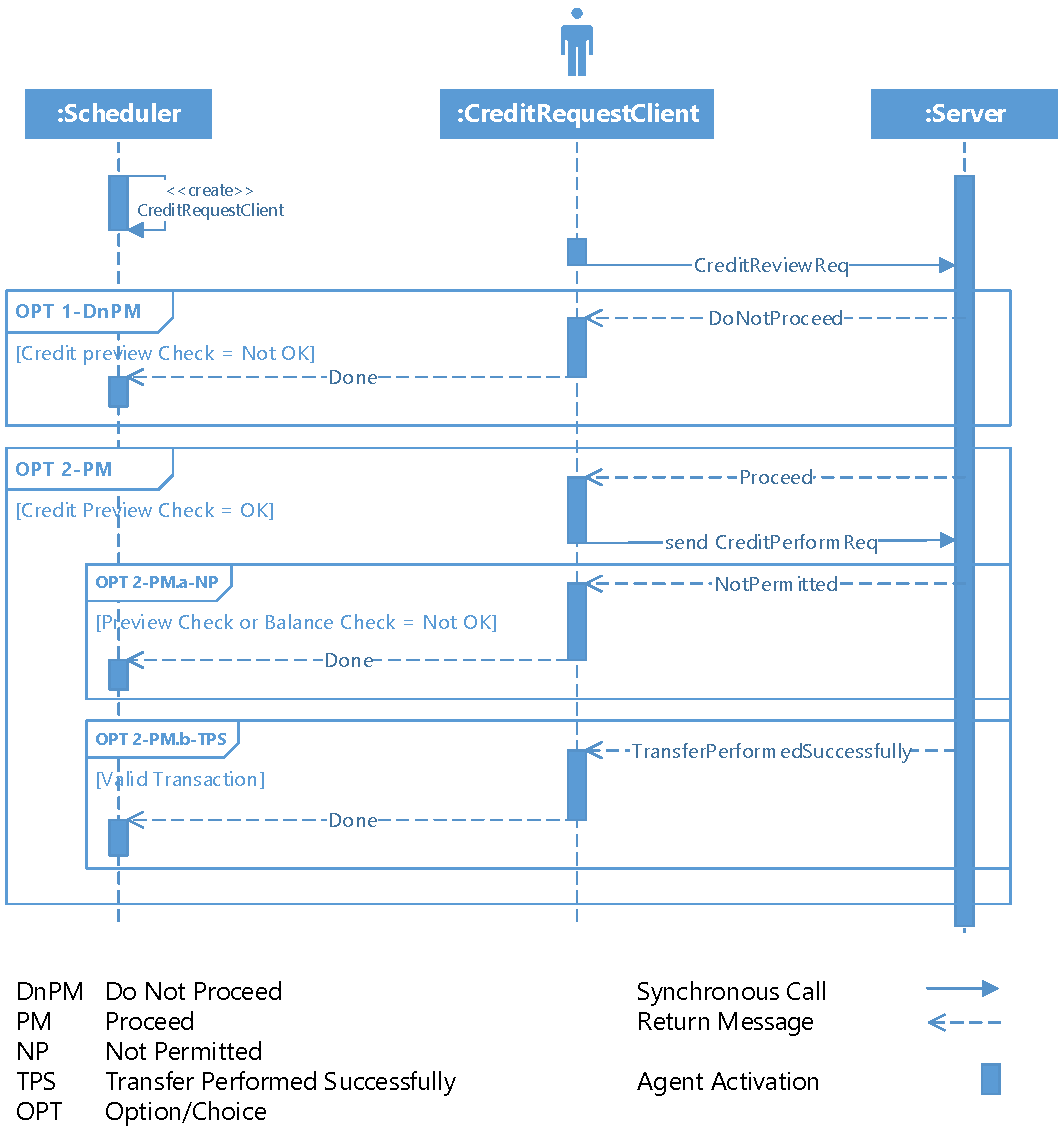
\includegraphics[width=1.0\textwidth]{Figures/creditrequest}
  \caption{\bf\small Credit request message protocol}
  \label{fig:impl-msg-crc}
\end{figure}


When following the sequence diagram in Figure \ref{fig:impl-msg-crc}, it is necessary to keep in mind that these messages are sent from a $CreditRequestClient$ but initiated and owned by a member who is logged in and registered in the session's data lookup table. For the server agent process it is important to know which member is currently sending that transfer in order to perform various checks and store valid transfers. Certainly, the same applies for the $DebitRequestClient$ and the $DebitAcknowledgeClient$ of Figure \ref{fig:impl-msg-drc}.

\textcolor{red}{``Do not proceed the message'' does not make sense in English. Perhaps you mean ``Do not forward the message"? If so, can you please change the two figures below and also the code? I.e. DoNotProceedMessage should become DoNotForwardMessage.}



\textbf{Dynamic Request Clients} start off when they are created by the $scheduler$ agent and do not send or receive any request beforehand. Consistently with a typical state machine, the clients manage their own states and act according to them. CRC\footnote{Credit Request Client} and DRC \footnote{Debit Request Client} use four main states that are explained in detail in Section \ref{subsec:impl-states}.

The message sequence from client to server is specified in Section \ref{fig:impl-msg-crc} for the CRC and in Section \ref{fig:impl-msg-drc} for the DRC. In comparing those two figures, it is clear that the message sequences look very similar: only the names vary by their prefix (debit versus credit). However, what might not be obvious here is that the request parameters are quite different.

Another main difference between the credit and debit message sequences is, though, that a debit request needs $ConfirmationReq$ as well as $DebitAckMsg$. This is necessary because an initiating creditor (Seller) needs to have the transaction confirmed by the debtor (Buyer) to be sure of having a valid transaction which credits the payment to the Seller's own account.

\begin{figure}[htbp]
  \centering
  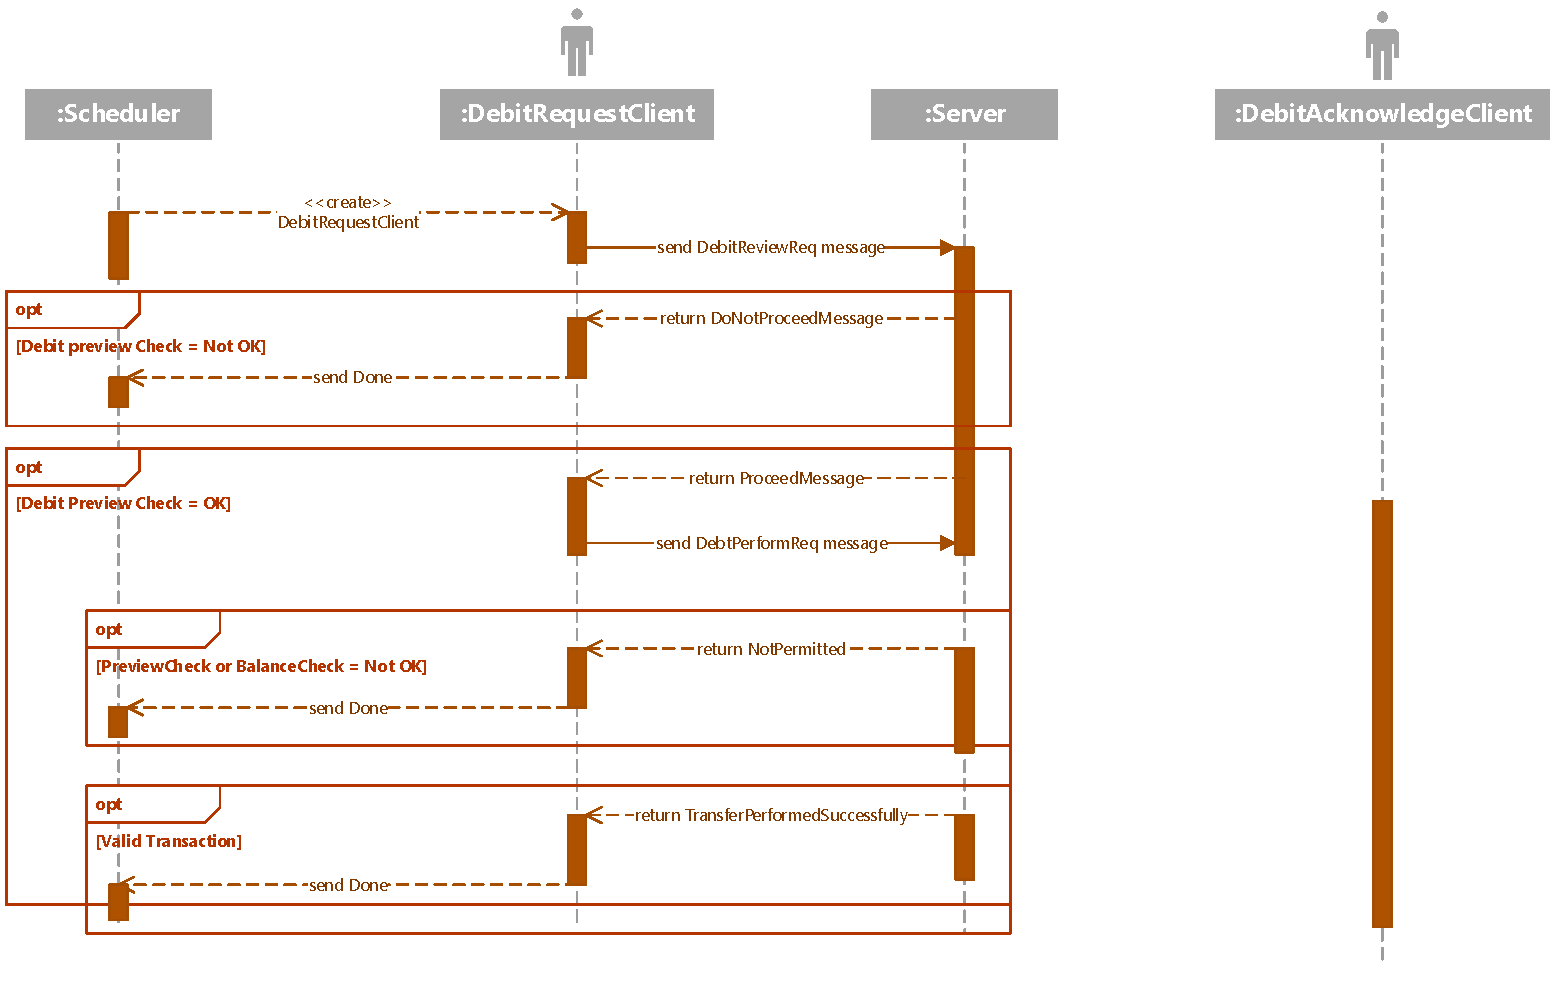
\includegraphics[width=1.0\textwidth]{Figures/debitrequest}
  \caption{\bf\small Debit request message protocol}
  \label{fig:impl-msg-drc}
\end{figure}

The sequence diagrams denote optional flows using option boxes. These boxes have a unique, numbered name. An option $OPT$ at the first level has a number (choice $1$ or $2$) as well as an abbreviated name ($DnPM$, $PM$). Sub-options in the second level are alphabetically numbered and also followed by an abbreviated name. Square brackets underneath the option name indicate the current option choice.

\textcolor{red}{It is not clear to me what `to reduce the executed command to a minimum' means. Even if I "fix" it as `to reduce the number of executed commands to a minimum' I am still not entirely clear what you mean. Sure, decreasing the number of commands executed would slow things down, but with a GHz processor what difference does that make?}

ASIMs currently do not have the possibility to sleep for some time or until an event has occurred. Nevertheless, agents are able to reduce the executed command in the current tick to a minimum, thereby achieving a similar result. Inside of the sequence diagrams, activated clients are shown by the vertical fully colored bars. Non-active phases are indicated by the vertical dashed lines.

The emulated users in the figures are pictured on top of the clients to show that requests are sent by particular members.

Scheduler and server are agents which can be seen as autonomous processes in the simulation. The scheduler mainly acts as an orchestration tool for testing purposes and will be removed for actually deployed applications, whereas the server agent needs to exist in a real-world scenario. Maybe not as a process running on a centralized server structure but when taking a real distributed scenario into account it will be implemented using some kind of smart contract running inside of a virtual machine in a blockchain environment.

\subsection{State Management}
\label{subsec:impl-states}

\subsubsection{Client States}\ are managed over four predefined pseudo-static locations, as follows:
\begin{itemize}
	\item SEND: only when sending a message
	\item RECEIVE: receive and directly respond to messages
	\item TERMINATE: end execution; send ``Done'' message
	\item DONE: everything is done; ready to be terminated
\end{itemize}
$SEND$ might be used if a sequence of messages is sent where no reply message is needed, or just to submit an initial message at start-up before going right into the $RECEIVE$ mode.

$RECEIVE$ waits for the messages and acts accordingly. When a message has been received and it is necessary to send a response it is done right in $RECEIVE$ mode without changing to $SEND$ mode.

$SEND$ and $RECEIVE$ states could be set alternately, but when the $TERMINATE$ state is applied \textcolor{red}{By `applied' do you mean `requested'?} the process of shutting down the agent has been started. Once the $DONE$ state is reached, even if not stopped yet by the scheduler, the client won't do anything useful anymore.

The DAC\footnote{Debit Acknowledge Client} uses the same states except for the $SEND$ state because it only needs to receive and confirm a transfer by using the given one-time \st{pad} \textcolor{red}{password}. The DAC is an example of the fact that not all of the states need to be covered by a client, which may be relevant when creating new clients.

\subsubsection{Server \& Scheduler States}\ are not technically a part of this section, since it is mainly about the dynamic clients. Nevertheless, a brief explanation of their states is given here to keep them together.

\underline{The server} does not have any particular mode or state management yet. It just waits for messages and when it receives one it processes it directly.

\underline{The scheduler} mainly has its test states, as mentioned in Section \ref{subsec:impl-agent-tasks}, and transitions from one test to another till there are no tests left. For each test the scheduler has two stages:
\begin{packed_item1}
\small
\item \textbf{First}, in the starting phase all the clients of that particular test are started and counted. Clients which should be part of one test state need to be defined as dynamic and appended to the scheduler by using the $include$ statement in the $run.icef$ definition.
\item Then, the scheduler in its \textbf{second} phase waits for as many $DONE$ messages as the number of clients that have been issued \textcolor{red}{[do you mean spawned, or instantiated?]}. Finally, when the client count is zero, the scheduler goes to the next test and starts that two-phase process again.
\end{packed_item1}


%%%%%%%%%%TODO%%%%%%%%%
\section{Logging}
\label{sec:impl-log}

The server agent needs to place many different status messages of different importance. In order to manage their occurrence, a simple logger has been added. The logger introduces five log levels:
\begin{enumerate}
	\item FATAL
	\item ERROR
	\item WARN
	\item INFO
	\item DEBUG
\end{enumerate}
These levels denote the different severities that can be \st{applied to} \textcolor{red}{recorded into} the logger and \st{define} \textcolor{red}{necessarily communicate} the maximum severity of a message presented to the executing user. To explain further, $FATAL$ messages should be printed always, whereas $DEBUG$ messages are only of interest for developers who need very detailed information of the current state.

Consequently, the maximum log level can be given at agent start-up inside of the $init$ rule. The rule used to define the level is explained here

\begin{lstlisting}[language=bsl]
	//rule header
	rule initCustomLogger(set_log_level) = ...
	...
	//init logger call
	initCustomLogger(DEBUG)
\end{lstlisting}

When initialized, the logger can be used at any place by calling the $do\_log$ rule, which takes two parameters. The first is the actual message printed to the output and the second parameter describes the importance of that message by using one of the five mentioned severity levels. The listing below shows first how to log a message with severity $INFO$ and the second call illustrates a $FATAL$ error message output.
	
\begin{lstlisting}[language=bsl]
	// An "INFO"-level message
	do_log("Transfer has been performed successfully", INFO)
	...
	// A "FATAL"-level error message
	do_log("List 'Ledger' in unknown state", FATAL)
\end{lstlisting}

Currently, the logger implementation can only be applied \textcolor{red}{utilized?} meaningfully inside of the server itself, because the implementation is also hosted by the server agent definition file $server.casim$ directly. It would certainly be possible to put the logger into a different file, but the $include$ statement of the $run.icef$ is not supported by the Eclipse plugin. Consequently, if the logger implementation were separated out into an additional file, all occurrences of $do\_log$ calls would be marked as erroneous (even if they were not) and would then turn the coding-assistance tools inside of Eclipse into an unusable environment.


\section{Test Scenario}
\label{sec:impl-test}

This deliverable does not cover the test management for the ICEF implementation of INTERLACE. However, in order to check if a base workflow of a requirement is working in its most simple form a strategy has been followed which has been partly explained already by other sections of this chapter. The scope of this section will therefore be to put these parts together and extend the missing bits.

\subsection{Separation of Concerns}

When looking at the environment from a testing perspective there are three parts which can be distinguished:

\begin{enumerate}
	\item Actual system requirements implementations
	\item Testing routines
	\item Simulation environment
\end{enumerate}

The "actual system requirement implementations" cover parts that are needed for a possible real-world system. Without these, the system would not be able to function. Therefore, they can be seen as the core part of the application which is entitled \textcolor{red}{[do you mean `supposed'?]} to be tested.

Second, code parts have been implemented which are only there for performing and validating a test of a particular scenario use case. Currently these scenarios are credit and debit operation requests sent from virtual clients.

Last, parts of the system had to be implemented in a prototypical and most basic form in order to achieve a very simple executable version which can accommodate the test scenarios. These parts were not included in the requirements definitions or in the refinements. These parts comprise implementation details not relevant to the requirements or to the main ledger implementation.

In Section \ref{subsec:impl-agent-tasks} the main agents are explained, $scheduler$ and $server$. When assembled for execution, they are fully implemented. The $server$ covers the actual system requirement realizations as well as the simulation environment code. To be more specific, the $server$ dispatches the message requests explained in Section \ref{lst:impl-msg-dispatch} and performs read actions to the virtual profile, account, etc. information, together with pushing transactions to a primitive ledger discussed in Section \ref{subsec:impl-sim-env}.

The $scheduler$ mostly contains testing routines but partly also routines that handle the necessary client implementations that are not covered by the requirements. The test routines are responsible for starting and destroying clients. As a short reminder, the $scheduler$ is able to do so because it also contains all the client code. Further, Listing \ref{lst:impl-msg-send} shows the sending of a test credit request issued by the $CreditRequestClient$. This message is processed by a challenge-respond 
\textcolor{red}{[Do you mean `challenge-response'?]} sequence between the server and the client that imitates a transaction.

Concluding, a correct execution is currently only shown by a client which outputs a transfer-performed message when done. In case of an error the client would provide a message indicating the cause.

\subsection{Simulation Environment}
\label{subsec:impl-sim-env}

The simulation environment created for enabling the core server parts to be executed and later be validated has an active and a passive part. The so-called active part takes care of storing a transaction into the ledger, while the passive part contains various pre-prepared locations which are needed to satisfy the different constraint requirements.

\subsubsection{Locations: }\ Beginning with the passive part, the following locations have been defined in the non-functional client $initdata$ shown in Listing \ref{lst:impl-sim-setup-locs}.

\begin{center}
\begin{minipage}{0.8\textwidth}
\small
\begin{lstlisting}[language=bsl_lst,caption={\bf\small Simulation environment locations},label={lst:impl-sim-setup-locs} ]
controlled TT: OPERATION * UNIT * USER_TYPE_GROUP -> SET
controlled AccT: OPERATION * UNIT * ACCOUNT_TYPES -> SET

controlled profileTable: MEMBER_ID -> MAP
controlled accountTable: ACCOUNT_ID -> MAP
controlled userGroupTable: MEMBER_ID -> USER_TYPE_GROUP
controlled sessionData: MAP
\end{lstlisting}
\end{minipage}
\end{center}

The two most important are the functional locations $TT$ and $AccT$. They correspond to the transfer type functions described in Section \ref{subsec:perm-trans-types} and the account connectivity conditions presented in Section \ref{subsec:perm-acc-con}, respectively. $TT$ was predefined precisely in the requirement definitions and is described as a functional mapping
\begin{asm}
TT: Operation \times Currency \times Group \rightarrow \{G \mid G \subseteq Group\}.
\end{asm}
So we can define that for a Credit operation in Sardex (SRD) an $Employee$ is allowed to perform a transaction with a member of the circuit which is part of one of the groups $Company$, $Retail$ or $Full$:
\begin{asm}
TT^{Credit,SRD}(Employee) =\{Company,Retail,Full\}.
\end{asm}
When translating this discrete functional mapping to BSL, the outcome looks like this:
\begin{lstlisting}[language=bsl]
	TT("credit", "SRD", "employee") := {"company", "retail", "full"}
\end{lstlisting}
The account connectivity function $AccT$ takes operation, currency, and account type as parameters and maps them to a group of account types:
\begin{asm}
AccT: Operation \times Currency \times AccountType \rightarrow \{Acct \mid Acct \subseteq AccountType\}.
\end{asm}
As discussed in full detail in the Appendix, when replacing the parameters by actual values we obtain:
\begin{asm}
\begin{array}{ll}
AccT^{Credit,SRD}(X) =\{ CC , Domu ,Mirror \} & \IF X \in CC,
\end{array}
\end{asm}
which then can be transformed again into the ``implemented'' form and is represented like this inside of the $initdata$ agent:
\begin{lstlisting}[language=bsl]
	AccT("credit", "SRD", "CC") := {"CC", "DOMU", "MIRROR"}.
\end{lstlisting}

The other locations listed in Listing \ref{subsec:perm-trans-types} \textcolor{red}{[I think you mean Listing \ref{lst:impl-sim-setup-locs}]} accommodate important information for groups, members, and sessions as well as accounts. Except for the $userGroupTable$, which just maps a user to its current operational group, all functions implement a result of type $MAP$. A $MAP$ is similar to a simple set with the difference that each entry of a $MAP$ is a key-value pair.

\begin{center}
\begin{minipage}{0.8\textwidth}
\small
\begin{lstlisting}[language=bsl_lst,caption={\bf\small $MAP$ example showing a profile table entry},label={lst:impl-sim-maps} ]
	//init profile data
	profileTable("mbrId1") := {
		"lowBalanceAlert" -> 700,
		"highBalanceAlert" -> 1000,		
		"highVolumeAlert" -> 10000,
		"capacity" -> 100000,
		"saleVolume" -> 50000,
		"accounts" -> ["accId1", "accId4"]
	}
\end{lstlisting}
\end{minipage}
\end{center}

Listing \ref{lst:impl-sim-maps} shows a typical definition of such a map which may be compared to a hash map used in various different other programming languages. Those values are accessed based on different pre-defined rules which are explained in Section \ref{sec:impl-rules}.

\subsubsection{Ledger: }\ The ledger but also the pending transactions are initialized as empty maps:
\begin{lstlisting}[language=bsl]
	Ledger := {->}
	PendingTransactions := {->},
\end{lstlisting}
and when a transaction matches the required constraints it is appended to that ledger map. For unconfirmed debit requests a second map called $PendingTransactions$ has been added which contains valid transactions which have not been confirmed by the debtor yet.

After the various checks -- which vary a little based to the type of operation -- have been passed successfully, the transaction is appended using the following command:
\begin{lstlisting}[language=bsl]
	Append(Transaction(transfer, client, "debit", now), Ledger)
\end{lstlisting}

A pending transaction awaiting a correct OTP from a debtor is added to location $PendingTransactions$ as follows:
\begin{lstlisting}[language=bsl]
	Insert(transfer, creditor, PendingTransactions) Ledger).
\end{lstlisting}

After a transaction has been confirmed by a valid OTP, it is moved, as mentioned, to the actual ledger. Inside the $PendingTransactions$ map the state of that transaction \st{receives state} \textcolor{red}{is changed to}
$TRANSACTION\_PERFORMED$ but the transaction is not deleted.

\subsection{Additional Login Layer}
\label{subsec:impl-login-layer}

The requirements \st{definitions} \textcolor{red}{specifications} do not define how authentication is handled by the system. Agents in ICEF have predefined names which cannot be changed during runtime. In order to act flexibly and reuse agents, a login layer has been introduced. Thus agents who are actively communicating with the server need to be registered in the $sessionData$ location which is initialized in the $initdata$ function.

Agents in the current prototypical implementation do not login by themselves by providing a username and password but place their address together with a valid member ID in the $sessionData$ MAP as shown here:
\begin{lstlisting}[language=bsl]
	sessionData := {
		"CreditRequestClient@CreditRequestClient" -> "mbrId1",
		"DebitAcknowledgeClient@DebitAcknowledgeClient" -> "mbrId4",
		"DebitRequestClient@DebitRequestClient" -> "mbrId2"
	}
\end{lstlisting}
The address of an agent is defined by ``<name>@<name>'', thus concatenating two occurrences of its own name with an ``@'' symbol. The address is taken during message processing. For example, when looking at the above $sessionData$ setup, it is possible to determine that agent CreditRequestClient's messages are sent by user mbrId1. \textcolor{red}{The syntax seems to suggest that agent CreditRequestClient's messages are sent TO user mbrId1, rather than BY. Can you explain a bit better the semantics of the arrows?}

The member ID represents an alphanumerical string assigned after first registration \textcolor{red}{Is there a second registration? If not, delete `first'; if Yes, then please explain how and why it (the second registration) takes place.} For the INTERLACE implementation this means that an entry also needs to exist in location $profileTable$, in addition to $userGroupTable$, at which point the user has been properly registered and is known to the system. If the user wishes to perform a transaction, for the transaction to be valid an entry in location $accountTable$ should be added for that user, \st{in order to assign and work with an actual account.}  \textcolor{red}{in order to assign an actual account to that user and enable the system to work with it.}

At runtime two derived functions are used to read the information of $sessionData$. As shown below, a member ID of an ``active'' user can be determined by calling $activeLogin$. Whether a member is currently logged in may be found out by obtaining the result of $activeClient$.

\begin{lstlisting}[language=bsl]
	//get member id by providing a client name using session information
	derived activeLogin(client_address) = ...
	//usage
	login_mbrId := activeLogin("CreditRequestClient@CreditRequestClient")
	
	//get client name by providing member id using session information
	derived activeClient(login_mbrId) = ...
	//usage
	client_address := activeClient("mbrId1")
\end{lstlisting}

One restriction needs to be mentioned though: a client address \st{only can have} \textcolor{red}{can only be associated with} one logged-in member at any one time, and vice versa.

\section{Important Rules and Locations}
\label{sec:impl-rules}

Next, the emphasis is put on explaining rules and locations not discussed in detail or not mentioned at all in this document yet. All rules and locations in this section can be \st{located} \textcolor{red}{found} in file $server.casim$ or $initdata.casim$, which is added to the server part \st{due to} \textcolor{red}{by means of} the $include$ statement in run.icef.

In the BSL \st{code} \textcolor{red}{language}, the $choose$ keyword is needed to read the content inside a map, 
\textcolor{red}{[Not clear what you mean by content ``inside'' a map. If by a map you mean a mathematical function, are you referring to the value of the function? If it is a function that is represented as a table, do you mean the contents of the table? Perhaps you can use more explicit language.]} which makes the code difficult to read in some cases. To simplify this access, we introduced a derived function $v$ for working with $MAP$-type locations:
\begin{lstlisting}[language=bsl,mathescape=true]
	$\Rightarrow$ derived v(amap, key).
\end{lstlisting}

The parameter $amap$ can be any $MAP$-type location and the $key$ refers to the entry of interest. Consequently, the corresponding $value$ can be read by passing an existing $key$, as illustrated in the following example:
\begin{lstlisting}[language=bsl,mathescape=true]
	mymap := {
		"thekey" => "assignedvalue",
		"another" => "somevalue"		
	}
	valueofkey := v(mymap, "thekey")
\end{lstlisting}
Finally, if the map or the key is undefined, also the result will be.

The ICEF framework uses a plugin called ``CommunicationPlugin'' to establish a simple communication system. As mentioned in the previous section, a method called $send$ is used to transfer a message \textcolor{red}{between ASIMs}. However, the server implementation usually does not call that method directly but, rather, it calls a rule with the same name starting with an upper-case letter. This $Send$ rule takes as first parameter a message which contains a list of two strings. The two strings are the message content itself and the message subject. In order to abstract the message type from the user, a derived rule called $AssembleMessage$ is provided for creating such a message. The second parameter is the recipient agent's name, not a member with a particular ID: \textcolor{red}{[do you mean to say `not the ID of a particular member'?]}
\begin{lstlisting}[language=bsl,mathescape=true]
	$\Rightarrow$ derived AssembleMessage(msg, sub)	
	$\Rightarrow$ rule Send(msg, agent).
\end{lstlisting}

When passing a message before sending, other parts of the implementation may use the functions $messageContent$ and $messageSubject$ on the assembled message to get back the content and the subject, respectively. Also $Send$ uses these two functions to read content and subject for the actual sending process. In case of error or success, corresponding response messages are generated. $IncorrectOtpFor$ is one example which is used inside the $server$ implementation to create an appropriate error message based on particular related arguments:
\begin{lstlisting}[language=bsl,mathescape=true]
	$\Rightarrow$ derived messageContent(msg)
	$\Rightarrow$ derived messageSubject(msg)
	$\Rightarrow$ derived IncorrectOtpFor(otp, amount, creditor).
\end{lstlisting}

Continuing further on OTPs, there are three important functions that should be mentioned in addition to the requirement definitions. $RandomHex$ generates a random hexadecimal number. Next, $HexString$ calls $RandomHex$ $n$ times, where $n$ equals the first parameter $length$ \st{resulting in} \textcolor{red}{in the form of} a hexadecimal string. This hexadecimal string generation is used for creating OTPs as well as transaction IDs for appending unique transactions to the ledger:

\begin{lstlisting}[language=bsl,mathescape=true]
	$\Rightarrow$ derived RandomHex
	$\Rightarrow$ derived HexString(len)
	$\Rightarrow$ derived OneTimePassword(strength)
\end{lstlisting}

Transactions are transferred using a $MAP$. A credit transfer is shown next:
\begin{lstlisting}[language=bsl,mathescape=true]
	$\Rightarrow$ CREDITREQUEST := {
			"from" -> "accId1",
			"to" -> "accId2",
			"channel" -> "Service",
			"amount"  -> 2000,
			"metadata" -> {"message", "some transfer"}
	  }	
\end{lstlisting}

For all attributes used inside these transfer-request maps, derived functions have been created. One function and its usage is shown here:
\begin{lstlisting}[language=bsl,mathescape=true]
	$\Rightarrow$ derived fromAcc(transfer)
	// example
	fA := fromAcc(CREDITREQUEST)
	fA = "accId1" //is true
\end{lstlisting}

Next, we examine the ledger and the preliminary storage for pending transactions. Both are maps storing transactions. The difference is that \textcolor{red}{the function} $PendingTransactions$ is using an OTP key to map to a transaction, whereas a finally persisted transaction is mapped using an transaction ID key. \st{One-time pads} \textcolor{red}{OTPs} are created by $OneTimePassword$ and transaction IDs are created by calling $NewTransactionID$.

\begin{lstlisting}[language=bsl,mathescape=true]
	$\Rightarrow$ controlled Ledger: MAP
	$\Rightarrow$ controlled PendingTransactions: MAP
\end{lstlisting}

Rule $Insert$ adds a transaction which awaits confirmation \st{to} \textcolor{red}{[either `for' or `from']} a map which needs to be the last parameter. The $server$ stores all these unconfirmed requests in the map $PendingTransactions$, as indicated above.

After a valid and existing OTP has been sent for a transfer in $PendingTransactions$, the transfer needs to undergo some more checks; but, when \st{passed} \textcolor{red}{approved}, it is appended to the Ledger by executing the rule $Append$.

$Insert$ and $Append$ are listed here together with $Transactions$ and $NewTransactionID$:\\
\textcolor{red}{[What's the difference between `trans' and `transfer'?]}
\begin{lstlisting}[language=bsl,mathescape=true]
	$\Rightarrow$ rule Append(trans, ledger)
	$\Rightarrow$ rule Insert(transfer, creditor, pendingTransactions)
	$\Rightarrow$ derived NewTransactionID(len)
	$\Rightarrow$ derived Transaction(transfer, mbr, operation, date)
\end{lstlisting}

Finally, we described a rule that is part of the requirements but is used in a different way. The requirements call for three functions called $FinalDebitAccountLimitsCheck$, $DebitAccountLimitsCheck$, and $CreditAccountLimitsCheck$. These functions are similar and \st{are used in a consolidated way for} \textcolor{red}{are integrated in} the ICEF implementation. $PreviewCheck$ implements this check and needs the member ID $mbr$, the $from$ account $fromA$, the $to$ account $toA$, a $from$ group $fromGroupId$, a $toGroupId$ and, as last parameter, the operation $operation$ as a String. The operation string can be either ``credit'' or ``debit''. This code example shows the rule but also how it is used in the current setup:

\begin{lstlisting}[language=bsl,mathescape=true]
	$\Rightarrow$ rule PreviewCheck(mbr, fromA, toA, fromGrpId, toGrpId, operation)
	//example: do check the transfer if it is ok
	error <- PreviewCheck(
		activeLogin(client), //read mbr from message client-address
		fromAcc(transfer), //read from account of transfer
		toAcc(transfer), //read to-account of transfer
		groupOf(ownerOf(fromAcc(transfer))), //get group of from-account owner
		groupOf(ownerOf(toAcc(transfer))), //get group of to-account owner
		"credit" //Operation as string
\end{lstlisting}

The result of $PreviewCheck$ is either $undef$, if all checks are successful, or it contains a textual message indicating the problem.

\section{Implementation Challenges}
\label{sec:impl-challenges}

When working with the ICEF framework, some things should be noted. Currently, the ICEF framework is an academic tool and not ready for industry use. Additional effort needs to be expended in order to achieve a fully integrated system for an industry-grade software design process or even a continuous integration process. \textcolor{red}{We now outline some of the still-open issues.}

\subsection{Issues}

During development the team has been confronted with different issues regarding the ICEF framework but also with the process of moving the specifications to a running ASIM INTERLACE Model:
\begin{description}
	\item[Unknown line numbers] Before transmitting a simulation to the ICEF manager, JavaScript code loads all specified .casim files, preparing them for being sent over the network in the form of a consolidated JSON message. This process, together with the added preliminary $include$ syntax, \st{cause} \textcolor{red}{exhibits} a problem with respect to error messages. More precisely, if something goes wrong the error messages do not contain the relevant line number(s) of where the error occurred. Thus, in case of any failure it can be very difficult to locate the actual cause.
	\item[Error in block] Errors inside a block cause the whole block not to be executed for unknown cases. \textcolor{red}{[Do you mean `for unknown reasons'?]} For example, if a block has $n$ statements and the last one has a problem, all the other $n - 1$ statements might not be executed either, even if a sequential block was used. Given that the error messages do not contain correct line numbers, finding a problem with debug output to the console also does not work appropriately in all cases.
	\item[Parallel blocks] ASM code and consequently also BSL code allows to write so-called parallel blocks. These blocks start with $par$, end with $endpar$, and contain code which is executed in parallel -- at least theoretically. The important thing to know here is that the order of execution is not guaranteed. This can lead -- and actually led during development -- to unpredictable behaviour and needs to be used with caution!
	\item[Bugs] As the ICEF framework is still at the alpha stage, a couple of bugs occurred which could be fixed. However, further testing iterations are needed to make the framework stable.
	\item[Testing] Various testing approaches still need to be investigated, because at the moment only the text output of a simulation can be checked to test if the system is running correctly. These testing approaches will be part of the upcoming research.\footnote{For example, we are likely to adopt Cucumber \url{https://cucumber.io/} and Gherkin \url{https://docs.cucumber.io/gherkin/}, since they are used by the Hyperledger blockchain development community.}
	\item[Modules] The solution of how modules, or how other code snippets, are integrated comes with strings attached, like the inaccurate/missing line numbers mentioned above and duplicated name spaces. Thus, a re-factoring for later use is highly recommended.
	\item[From document-based to executable] When a system behaviour has been written down in the form of an ASM/ASIM specification, it is necessary to note that a direct translation to ASM/BSL code is not always straightforward. One reason is that the functions and rules are not consistently available for CoreAS(I)M, and a lot of code for ``getting it to run'' needs to be worked out.
\end{description}

\subsection{Current Status}

The requirements for credit and debit operations have been implemented and are ready for more sophisticated tests. Also the base conditions for including further operations or requests handled by the server can be easily extended.

A test scenario has been built which may be used later for high-level testing, where particular use cases are played through using a predefined set of tests including agents with particular tests.

B2C-operations and also some of the other requests defined like $AccountHistReq$ still need to be taken care of and will be addressed in future work.









